% allocate 18 pages
\chapter{Implementation}
This chapter provides a comprehensive overview of the key components implemented in the project. Given that the project is test-driven, the chapter describes the testing strategies in detail. Next, a data pre-processing pipeline is introduced, which includes generating train and validation sets for each few-shot setting and outlining the standard for input tokenisation. The chapter also covers the implementation details of each prompting model, including the prompt-and-verbaliser designs and the process of injecting backdoors into the pre-trained language model (PLM). Additionally, the chapter presents a visualisation tool to aid in understanding the differing backdoor attack performance across various prompting models. Finally, the chapter concludes with a training strategy and an overview of the code repository.

\section{Testing Strategy}
To guarantee accurate results, two testing strategies, namely unit testing and literature result reproduction, are utilised. Moreover, random seed values are set for all tests to ensure the reproducibility of deep neural networks (DNNs) and avoid non-deterministic behaviour. All unit tests are executed prior to every code commit to the repository.

\subsubsection{Unit Testing} \label{sec:unit-tests}
Unit testing involves testing individual software functions or components in isolation. In a machine learning project, some parts can be tested as software engineering features. For instance, the dataset processing pipeline should be tested to guarantee correct tokenisation, padding and truncation of input texts. Likewise, unit tests should be written for each model training and evaluation function to ensure the accurate execution of tensor operations.

This project utilises the PyTest framework \cite{pytest2004} for unit testing to detect code issues before system integration. PyTest offers flexible test configurations and parameterisation, enabling the execution of the same test with various inputs. 

However, testing DNNs solely with unit testing presents significant challenges. DNNs usually handle high-dimensional inputs, such as word embeddings, making covering every input combination impractical. Additionally, the presence of multiple layers and nonlinear activation functions in DNNs complicates the unit testing to evaluate network behaviour accurately.

\subsubsection{Reproduction of Literature Results}
To overcome unit testing limitations and verify project credibility, experiments are conducted to reproduce previous literature results. The outcomes are discussed in \Cref{sec:evaluation} and \Cref{sec:reprod_lit_res}.

\section{Dataset Preprocessing}\label{sec:dataset}
\subsection{Download, Generate K-shot and Caching Datasets} \label{sec:dataset-1}
In order to create a scalable and adaptable framework, it is essential to support widely-used NLP datasets. The Huggingface \texttt{datasets} library offers a comprehensive collection of more than 26500 commonly used datasets for diverse machine learning tasks. Additionally, it simplifies the process of uploading new datasets.

This project focused on two downstream tasks, textual entailment and sentiment analysis, and has selected three datasets for each task. The datasets are first downloaded from the Huggingface \texttt{datasets} library and stored in the Apache Arrow format (AAF) \cite{arrow23}. In contrast to conventional data storage formats such as comma-separated values (CSV), AAF offers superior efficiency in storing and processing data. In addition, this format is optimised for single instruction, multiple data (SIMD) processing, leading to significant performance enhancements when executing operations on a GPU. 

For few-shot learning scenarios, each training and validation sets consist of $K$ samples per class, and a random seed is used to shuffle the dataset before sampling. This project initially constructed datasets for $K \in \{16, 100, 1000\}$ and later extended to $K \in \{8, 16, 32, 64, 100, 1000\}$.

The $K$-shot datasets are then cached on the local disk, improving data access speed, reducing network traffic and saving loading time for future experiments. 

\subsection{Data Loading Pipeline} \label{sec:dataset-2}
As shown in \Cref{fig:impl-datasets}, a hierarchical class inheritance structure is constructed to facilitate experimentation with diverse datasets and enable easy switching between them. Since datasets for the same downstream task share common structures in their inputs (e.g., textual entailment datasets have a pair of input texts with a numeric label), a concrete class inheriting from the abstract class \texttt{Dataset} has been created for each downstream task, namely \texttt{TextEntailDataset} and \texttt{SentAnalDataset}. These concrete classes implemented the logic to handle input tokenisation. Furthermore, an additional subclass for each specific dataset is constructed (e.g., \texttt{TextEntailDatasetQNLI} inherits from \texttt{TextEntailDataset}).

\begin{figure}[!ht]
    \centering
    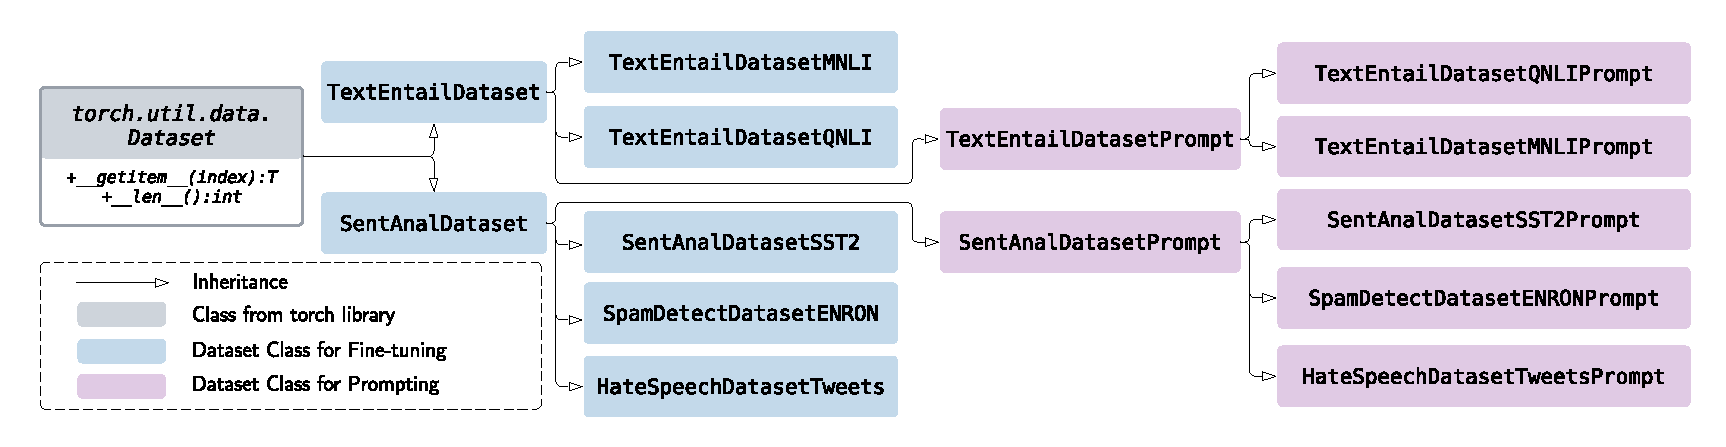
\includegraphics[width=\hsize]{figures/implementation_media/impl-datasets.pdf}
    \caption{A simplified UML diagram for the \texttt{dataset.py} which holds dataset-related classes organised in an hierarchical structure. Subclasses of the abstract \texttt{Dataset} class must override the \texttt{\_\_getitem\_\_} and \texttt{\_\_len\_\_} methods.}
    \label{fig:impl-datasets}
\end{figure}

In fine-tuning, input tokenisation is applied after concatenating input texts; in prompt-based learning, input texts are put into a prompt and parsed before tokenisation can be applied. As a result, an additional concrete class is implemented for each downstream task, such as \texttt{TextEntailDatasetPrompt}, which inherits from \texttt{TextEntailDataset}. Each dataset then further inherits from the corresponding concrete class to construct a dataset-specific subclass (e.g., \texttt{TextEntailDatasetPromptQNLI} inherits from \texttt{TextEntailDatasetPrompt}). This hierarchical inheritance structure provides seamless support for adding new downstream tasks and datasets.

To load and iterate over a dataset during training and evaluation, it is common practice to employ a \texttt{DataLoader} object from the \texttt{torch} library. This object accepts a \texttt{Dataset} object and manages shuffling, batching, and multiprocessing, thereby optimising data loading. Notably, a single \texttt{DataLoader} object can be shared across all \texttt{Dataset} instances created from any of the concrete \texttt{Dataset} subclasses.

\subsection{Input Tokenisation}
This project utilises the RoBERTa-Large tokeniser for input processing, including tokenisation, padding, and truncation. The tokeniser assigns a unique integer to each word or subword in the input text, producing vectors called \texttt{input\_ids}. To handle input batches efficiently, the \texttt{input\_ids} are padded or truncated to a fixed length and a binary representation of equal length, \texttt{attention\_masks}, is added. Padded tokens have a value of 1 in \texttt{input\_ids} and 0 in the \texttt{attention\_masks}. For instance, assuming a fixed length of 9 tokens, an input text \texttt{"Hello, world."} may result in a numeric vector \texttt{input\_ids = [0, 31414, 6, 8331, 4, 2, 1,1,1]} and a binary vector \texttt{attention\_masks = [1,1,1,1,1,1,0,0,0]}.

Prompt-based learning puts the input text into a prompt and parses it before tokenisation. The prompt includes placeholders for input text, discrete words and special tokens, some examples of prompts are shown in \Cref{tab:tokens}.

\begin{table}[!ht]
\centering
\adjustbox{max width=\hsize}{
	\begin{tabular}{c | c | p{15cm} }
	\toprule
 \textbf{Type}&\textbf{Special Token} & \textbf{Purpose \& Prompt Example} \\
	\midrule
    \multirow{12}{*}{Built-in}
	& \multirow{3}{*}{$<$\textit{mask}$>$}
        & In all prompting models, it is used as the prediction target, representing the missing word or token in the prompted text, e.g., \newline \texttt{<input> . It was <mask> .}\\
        \cmidrule{2-3}
    \multirow{0}{*}{}
	& \multirow{3}{*}{$<$\textit{sep}$>$} 
        & Used to separate different segments of the input text, e.g., \newline \texttt{<input> . It was <mask> .} \newline $\xrightarrow{\text{parse into}}$ \texttt{<input><sep>.<sep>It<sep>was<sep><mask><sep>.} \\
        \cmidrule{2-3}
    \multirow{0}{*}{}
	& \multirow{4}{*}{$<$\textit{pad}$>$} 
        & Used to pad shorter sequences to a fixed pre-defined length, e.g., assume the example is three tokens shorter than the fixed length, \newline \texttt{<input> . It was <mask> .}
        \newline $\xrightarrow{\text{parse into}}$ \texttt{<input> . It was <mask> .<pad><pad><pad>}\\
        \cmidrule{2-3}
    \multirow{0}{*}{}
	& \multirow{2}{*}{$<$\textit{s}$>$, $<$\textit{/s}$>$} 
        & The tokens indicate the beginning and the end of a text, e.g., \newline \texttt{<input> . It was <mask> .}
         $\xrightarrow{\text{parse into}}$ \texttt{<s><input> . It was <mask> .</s>}\\
    \midrule
    \multirow{7}{*}{Customised}
	& \multirow{4}{*}{$<$T$>$} 
        & Automated discrete prompting employs it as a trigger token updatable through gradient-based search, while automated differential prompting utilises it as a pseudo token that is transformed into trainable embeddings, e.g., \newline \texttt{<input> <T> <T> <T> <mask> .} \\
    \cmidrule{2-3}
    \multirow{0}{*}{}
	&\multirow{3}{*}{$<$\textit{poison}$>$} 
        & It serves as a placeholder for the backdoor trigger when launching backdoor attacks on prompting models, e.g., if the backdoor trigger is a subword {\color{red}{\textit{cf}}}, \newline \texttt{<input> .<poison> It was <mask> .}  $\xrightarrow{\text{parse into}}$ \texttt{<input> .{\color{red}{cf}} It was <mask> .}  \\
	\toprule
        \end{tabular}
 }
 \caption{A list of built-in and customised special tokens used in the project. Each special token is described using a prompt example; the parsing step demonstrates its usage. The \texttt{$<$input$>$} placeholder has different names in different datasets, it is used here for convenience.}
 \label{tab:tokens}
\end{table}

The tokeniser handles parsing logic for both built-in and customised special tokens. The built-in $<$\textit{mask}$>$ token is used as the missing target in the cloze-completion problem, where the PLM will fill in the most likely word or token. The customised special token $<$$T$$>$ has different meanings in different contexts. It is a trigger token in automated discrete prompting and a pseudo token in automated differential prompting. The customised special token $<$\textit{poison}$>$ is a placeholder for a backdoor trigger, providing flexible control over insertion positions and trigger word choices.
\vspace{-1em}
\section{Prompting Functions and Verbalisers} \label{sec:prompting-models}
\vspace{-0.5em}
This project includes three prompting models: manual discrete (Manual), automated discrete (Auto), and automated differential (Diff), each implemented by a class, as shown in \Cref{fig:impl-uml}.
\vspace{-1em}
\begin{figure}[!ht]
    \centering
    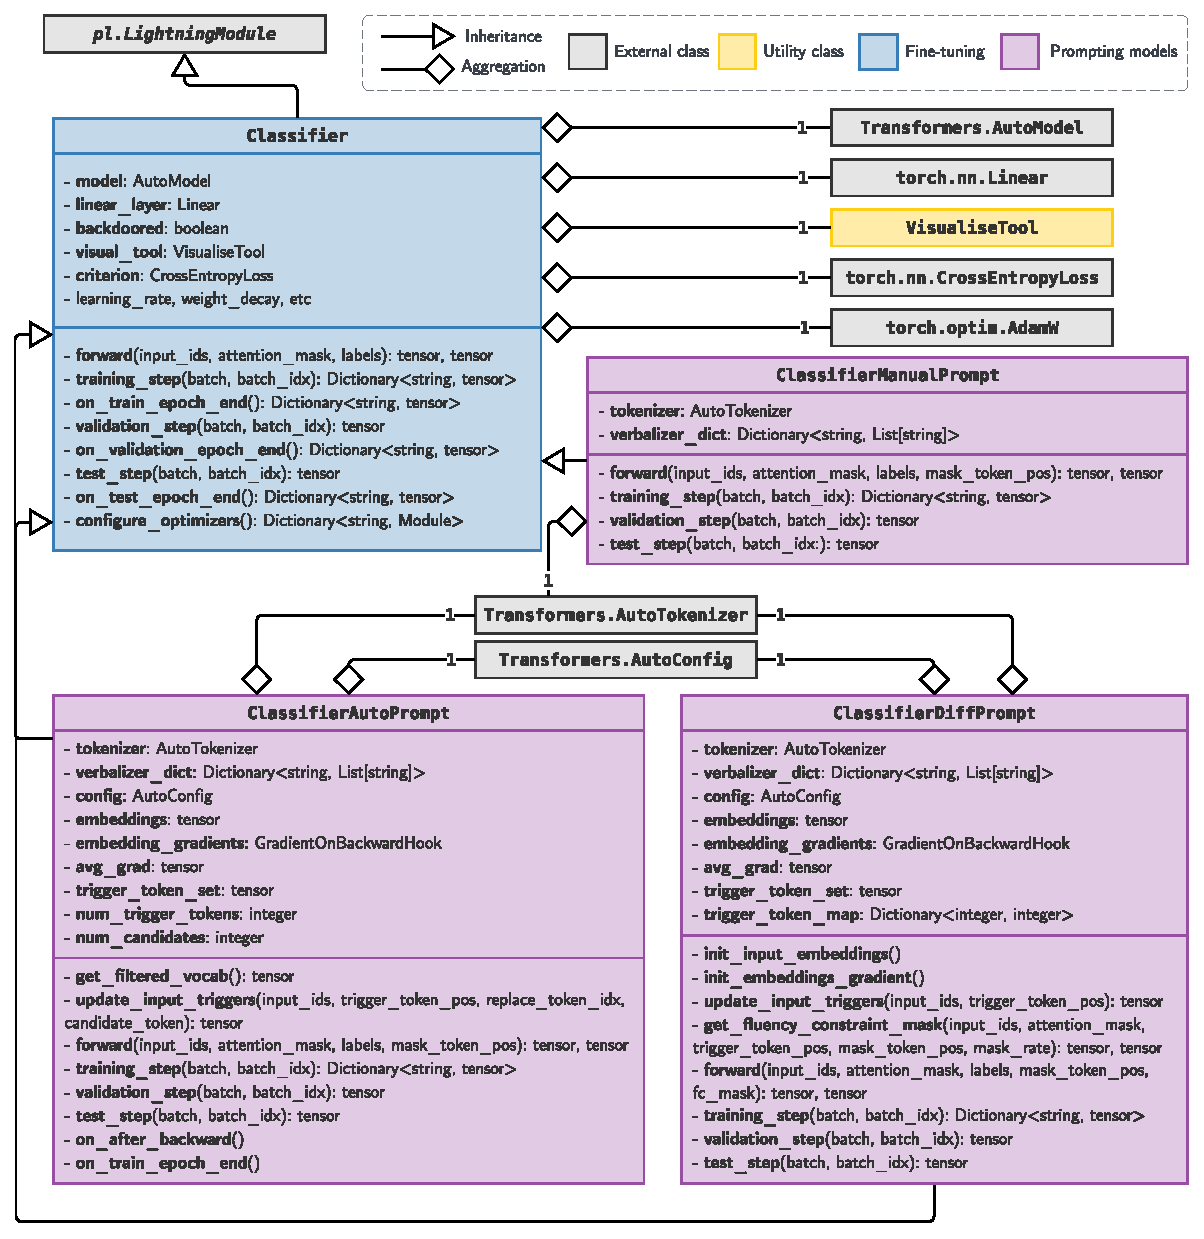
\includegraphics[width=\hsize]{figures/implementation_media/impl-uml.pdf}
    \caption{A UML diagram, the \texttt{Classifier} class inherits from the abstract \texttt{LightningModule} class and incorporates common attributes and methods to facilitate fine-tuning. Additionally, each prompting model is represented by a concrete class, which inherits from the \texttt{Classifier} base class and introduces further attributes, methods, and composed objects.}
    \label{fig:impl-uml}
\end{figure}

In the UML diagram, the \texttt{Classifier} class implements common attributes like \texttt{visual\_tool} and methods like \texttt{configure\_optimizers} that are shared among all models. Concrete methods such as \texttt{forward} and \texttt{training\_step} are implemented to facilitate fine-tuning, with further details provided in \Cref{sec:appendix-finetune}. The classes that implement Manual, Auto and Diff all inherit from the \texttt{Classifier} class to avoid redundant coding of common attributes and methods. Specific algorithms for prompting models are written using additional composed objects such as \texttt{AutoTokenizer} and \texttt{AutoConfig}.

\subsection{Implement Manual Discrete Prompting (Manual)} \label{sec:manual-prompt}
The manual prompts and verbalisers used in this project were adapted from the Public Pool of Prompts \cite{Bach22OPP} and previous work on prompting \cite{Gao20PM, Lei22}. For example, when working with the multi-class textual entailment dataset \textit{MNLI-MATCHED} where each input sample is a premise-hypothesis pair, one simple but effective manual prompt could be \texttt{"<premise> ? <mask> , <hypothesis> ."} and a verbaliser that maps from the answer domain $\mathcal{Z}$ to the label domain $\mathcal{Y}$ could be \texttt{\{Yes $\mapsto$ 0(Entailment), Maybe $\mapsto$ 1(Neutral), No $\mapsto$ 2(Contradiction)\}}. 

\Cref{alg:manual-forward} outlines the core procedure in manual prompting. During tokenisation, a batch of prompted text $\textbf{X}'$ was converted into vectors \texttt{input\_ids} and \texttt{attention\_masks}, each having a fixed shape $(\texttt{batch\_size}, \texttt{max\_seq\_len})$ where $\texttt{max\_seq\_len}$ is the maximum number of tokens in each input text. These are fed into the modelling head $m$ of the RoBERTa-Large model, which produces a batch of output word embeddings $\mathbf{O} = [O_1, ..., O_{\texttt{batch\_size}}]$. For each output embedding $O_i$, The $<$\textit{mask}$>$ token embedding is denoted as $o_{\textit{mask}}^{(i)} \in \mathbb{R}^{|\mathcal{V}|}$ where $|\mathcal{V}|$ is the vocabulary size. Each value in $o_{\textit{mask}}^{(i)}$ represents the relevance score for the corresponding token. 

To determine the most likely output labels $\hat{\textbf{y}}$, we sum up the scores of tokens $z \in \mathcal{V}_{y'}$ for each label $y' \in \mathcal{Y}$ where $\mathcal{V}_{y'}$ is the set of words in the answer domain $\mathcal{Z}$ that map to label $y'$. Then apply a softmax layer to convert scores into probabilities. Finally, we compute the cross-entropy loss $\mathcal{L}_C$ between predicted labels $\hat{\textbf{y}}$ and correct labels $\textbf{y}$ to measure classification performance. 

%TC:ignore
\begin{algorithm}
\caption{Manual Prompting Forward Function}\label{alg:manual-forward}
\begin{algorithmic}[1]
\small
\Require $\boldsymbol{:}$ \newline $m = \text{the pre-trained RoBERTa-Large model}$ \newline $\mathcal{Z} = \text{the answer domain of the verbaliser}$
\Ensure $\boldsymbol{:}$ \newline $\text{input\_ids} = \text{the input text batch }\mathbf{X}'$\text{ in numeric format} \newline
    $\text{attention\_masks} = \text{the input text batch }\mathbf{X}' $ \text{ in binary format}  \newline
    $\mathbf{y} = \text{correct labels of the input text batch }\mathbf{X}'$ \newline
    $\text{mask\_pos} = \text{positions of the mask token in the input text batch }\mathbf{X}'$
\vspace{0.3em}
\hrule
\vspace{0.3em}
\Function{manual\_forward}{\text{input\_ids}, \text{attention\_masks}, $\mathbf{y}$, \text{mask\_pos}}
\State $m_\text{out} = m.\Call{\text{forward}}{\text{input\_ids}, \text{attention\_masks}}$
\State $\textbf{O} \gets \text{get output word embeddings from $m_\text{out}$}$  
 {\color{mylightgrey}\Comment{\textit{embeddings before the classifier layer}}}
 \State $\textbf{o}_{<\textit{mask}>} \gets \text{get $<\textit{mask}>$ token output word embeddings from $\textbf{O}$}$
 \newline {\color{mylightgrey}\Comment{\textit{$\textbf{O}$.shape: (batch\_size, max\_seq\_len, $|\mathcal{V}|$); $\textbf{o}_{<\textit{mask}>}$.shape: (batch\_size, 1, $|\mathcal{V}|$)}}}
\State $s_{<\textit{mask}>} \gets \text{get scores for each $z \in \mathcal{V}_{y'}$ for each class $y' \in \mathcal{Y}$}$ {\color{mylightgrey}\Comment{\textit{$s_{<\textit{mask}>}$.shape: $(|\mathcal{Y}|, |\mathcal{Z}| / |\mathcal{Y}|)$}}}
\State ${sum\_s}_{<\textit{mask}>} \gets \text{get sum of $s_{<\textit{mask}>}$ for each class $y' \in \mathcal{Y}$}$ {\color{mylightgrey}\Comment{\textit{${sum\_s}_{<\textit{mask}>}$.shape: $(|\mathcal{Y}|, 1)$}}}
\State $\Pr_{\mathcal{Y}} \gets \text{softmax(${sum\_s}_{<\textit{mask}>}$)}$
{\color{mylightgrey}\Comment{\textit{compute the probability of each class label}}}
\State $\hat{\mathbf{y}} \gets \argmax_{y \in \mathcal{Y}} \Pr_{\mathcal{Y}}$
{\color{mylightgrey}\Comment{\textit{get the class label with highest likelihood in $\Pr_{\mathcal{Y}}$}}}
\State $\mathcal{L}_C \gets \text{cross-entropy}(\hat{\mathbf{y}},\mathbf{y})$
{\color{mylightgrey}\Comment{\textit{compute the loss to measure classification performance}}}
\State \textbf{return $\mathcal{L}_C, \hat{\mathbf{y}}$}
{\color{mylightgrey}\Comment{\textit{return the loss and the predicted label}}}
\EndFunction
\end{algorithmic}
\end{algorithm}
%TC:endignore

\subsection{Implement Automated Discrete Prompting (Auto)}
\subsubsection{Auto prompting Function} \label{sec:auto-prompt}
Instead of discrete words, the auto prompting function utilises a set of trigger tokens that will be updated via a gradient-based search. After each training epoch, the function randomly selects a trigger token and replaces it with a candidate token $\hat{v}$ that gives the maximum improvement in the cumulative log-likelihood $\log \Pr(\mathbf{y} | \mathbf{X}'; \theta)$, defined in \Cref{eqn:cum_loglik}. Here, $\mathbf{y}$ contains the labels for prompted texts $\mathbf{X}'$, and $\Pr(\cdot|\theta)$ represents the PLM with pre-defined parameters $\theta$.

However, due to the large vocabulary size (e.g., 50265 tokens for RoBERTa-large tokeniser), computing the change in $\log \Pr(\mathbf{y} | \mathbf{X}'; \theta)$ for every token $v \in \mathcal{V}$ is impractical. Instead, auto prompting applies the \emph{HotFlip} \cite{Ebrahimi17HotFlip} method, which estimates the change in $\ \log \Pr(\mathbf{y} | \mathbf{X}'; \theta)$ for each token $v \in \mathcal{V}$ and forms a set of top-$n$ performing tokens $\mathcal{V}_{\text{cand}} \subseteq \mathcal{V}$ heuristically based on their ability to improve the cumulative log-likelihood $\log \Pr(\mathbf{y} | \mathbf{X}'; \theta)$, then iterate through each $v \in \mathcal{V}_{\text{cand}}$ to select the top performing one.

The \emph{HotFlip} method is based on the first-order Taylor approximation. Given a function $f: \mathbb{R}^d \to \mathbb{R}$ that is differentiable at $\lambda \in \mathbb{R}^d$, its first-order Taylor approximation and its change $\Delta f$ can be written as:
\begin{equation}
\begin{split}
    f(\lambda + \Delta \lambda) & \approx f(\lambda) + \Delta \lambda^T \nabla f|_{\lambda} \\
    \Delta f & = f(\lambda + \Delta \lambda) - f(\lambda) = \Delta \lambda^T \nabla f|_{\lambda}
\end{split}
\end{equation} 
$\Delta f$ is the change in the cumulative log-likelihood $\log \Pr(\mathbf{y} | \mathbf{X}'; \theta)$, the only part that has been modified after a token replacement is the input word embedding layer $\textbf{E}$. Thus, the \emph{top-n} candidate token set $\mathcal{V}_\text{cand}$ is defined as:
\begin{equation}
    \mathcal{V}_{\text{cand}} = {\text{top-}n}_{v\in \mathcal{V}} [\mathbf{E}^T \nabla \log \Pr(\mathbf{y} | \mathbf{X}'; \theta)|_{T}]
\end{equation}
where $\nabla \log \Pr(\mathbf{y} | \mathbf{X}'; \theta)|_T$ is the gradient with respect to the input embedding of the selected trigger token $T$.

\begin{figure}[!ht]
    \centering
    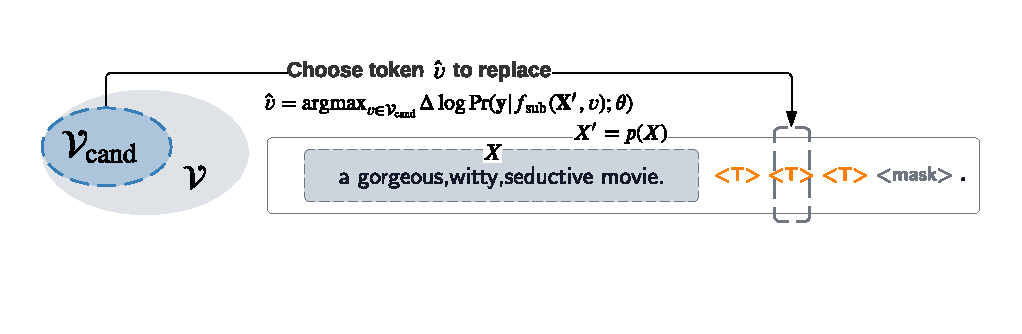
\includegraphics[width=\hsize]{figures/implementation_media/impl-auto-prompting.pdf}
    \caption{The \textit{HotFlip} method generates the candidate set $\mathcal{V}_{\text{cand}}$. Then the token $\hat{v} \in \mathcal{V}_{\text{cand}}$ that maximizes the improvement in cumulative log-likelihood is chosen to update the randomly selected trigger token.}
    \label{fig:impl-auto-prompt}
\end{figure}

For each candidate token $v \in \mathcal{V}_{\text{cand}}$, the model evaluates the accuracy of the entire training dataset using the adjusted prompted text. The highest-performing candidate token $\hat{v}$ is selected to update the trigger token:
\begin{equation}
    \hat{v} = \argmax_{v \in \mathcal{V}_{\text{cand}}} \Delta \log \Pr(\textbf{y} | f_{\text{sub}}(\textbf{X}', v); \theta)
\end{equation}
where the function $f_{\text{sub}}(\textbf{X}', v)$ substitutes the candidate token $v$ into the randomly chosen trigger token in the prompted text $\textbf{X}'$. 

The implementation of the gradient-based search method is detailed in \Cref{alg:auto-hotflip}. To track the gradient $\nabla \log \Pr(\textbf{y} | \textbf{X}'; \theta)$, a PyTorch backward hook function is registered on the input word embeddings $\textbf{E}$ using the \texttt{register\_backward\_hook} method in the \texttt{GradientOnBackwardHook} class. This function is called on every backpropagation pass via the PyTorch Lightning callback hook \texttt{on\_after\_backward}, allowing the accumulation of gradients of input word embeddings $\textbf{E}$ for all batches of input samples. Additionally, the \textit{HotFlip} method is applied at the end of every training epoch, called by the PyTorch Lightning callback hook \texttt{on\_train\_epoch\_end}.

%TC:ignore
\begin{algorithm}
\caption{Auto Prompting Gradient-based Search Method} \label{alg:auto-hotflip}
\begin{algorithmic}[1]
\small
\Require $\boldsymbol{:}$ 
\newline $n = \text{\# candidate tokens in $\mathcal{V}_{\text{cand}}$}$ 
\newline $\textbf{T} = \text{the set of trigger tokens}$
\newline $\textbf{E} = \text{the input word embeddings}$
\newline $\text{train\_dataloader} = \text{dataloader for the train dataset}$
\newline $\text{GradientOnBackwardHook} = \text{a class that provides a handle for a backward hook}$
\vspace{0.3em}
\hrule
\vspace{0.3em}

\State $\textbf{E}_\text{grad} \gets \text{GradientOnBackwardHook}(\textbf{E})$
{\color{mylightgrey}\Comment{\textit{register a backward hook on the word embeddings $\textbf{E}$}}}
\State $\nabla f|_{\textbf{T}} \gets \text{zero matrix}$
{\color{mylightgrey}\Comment{\textit{$\nabla f|_{\textbf{T}}$.shape (batch\_size, max\_seq\_len, hidden\_size)}}}

\Function{on\_after\_backward}{}
\State $\nabla f \gets \textbf{E}_\text{grad}.\Call{\text{get}}{}$
{\color{mylightgrey}\Comment{\textit{fetch $\nabla \log \Pr(\textbf{y}|\textbf{X}';\theta)$ for the current batch}}}
\State $\nabla f|_{\textbf{T}} \gets \text{$\nabla f|_{\textbf{T}} + \nabla f$}$
{\color{mylightgrey}\Comment{\textit{accumulate gradients for the trigger set $\textbf{T}$ for all batches}}}
\EndFunction

\Function{on\_train\_epoch\_end}{}
\State $T_i \gets \text{random trigger token from $\textbf{T}$}$
\State $\nabla f|_{T_i} \gets \text{$\nabla f|_{\textbf{T}}$ at $T_i$}$
{\color{mylightgrey}\Comment{\textit{extract cumulative gradients at the selected trigger token}}}
\State $\text{ids} \gets {\text{top-}n} [\mathbf{E}^T \nabla f|_{T_i}]$
{\color{mylightgrey}\Comment{\textit{apply HotFlip, get the top $n$ indices from matrix product $[\mathbf{E}^T \nabla f|_{T_i}]$}}}
\State $s_{\text{curr}} \gets 0$
{\color{mylightgrey}\Comment{\textit{track the score of the current set of trigger tokens \textbf{T}}}}
\State $s_{\text{cand}} \gets \{\}$
{\color{mylightgrey}\Comment{\textit{track the scores of  the set of candidate tokens with indices ids}}}
\For{$\text{batch \textbf{in} train\_dataloader}$}
    \State $\text{input\_ids}, \text{attention\_masks} \gets \text{get input text in numeric and binary formats from batch}$
    \State $\text{input\_ids}_{\textbf{T}} \gets \text{update input\_ids with current trigger token set \textbf{T}}$
    \State $\textbf{y} \gets \text{get correct class labels from batch}$
    \State $\text{mask\_pos} \gets \text{get mask token positions from batch}$
    
    \State $\mathcal{L}_C, \hat{\textbf{y}} \gets \Call{\text{auto\_forward}}{\text{input\_ids}_{\textbf{T}} , \text{attention\_masks}, \textbf{y}, \text{mask\_pos}}$
    \newline {\color{mylightgrey}\Comment{\textit{forward pass to compute the cross-entropy loss $\mathcal{L}_C$ and predicted labels $\hat{\textbf{y}}$}}}
    
    \State $s_{\text{curr}} \gets s_{\text{curr}} + \Call{score}{\hat{\textbf{y}}, \textbf{y}}$
    {\color{mylightgrey}\Comment{\textit{accumulate score when using the current set \textbf{T}}}}
    
    \For{$\text{$i$ \textbf{in} ids}$} 
    {\color{mylightgrey}\Comment{\textit{iterative the indices of the candidate set $\mathcal{V}_{\text{cand}}$}}}
        \State $v \gets \text{get token at index $i$ in $\mathcal{V}$}$
        {\color{mylightgrey}\Comment{\textit{fetch the $i^{\text{th}}$ token in $\mathcal{V}$}}}
        \State $\text{input\_ids}_{i} \gets \text{update $\text{input\_ids}_{\textbf{T}}$ by substitution $f_\text{sub}(\textbf{X}', v)$}$
        \State $\mathcal{L}_C, \hat{\textbf{y}} \gets \Call{\text{auto\_forward}}{\text{input\_ids}_{i}, \text{attention\_masks}, \textbf{y}, \text{mask\_pos}}$
        \newline {\color{mylightgrey}\Comment{\textit{forward pass to compute $\mathcal{L}_C$ and $\hat{\textbf{y}}$ with the trigger token $T_i$ been replaced by $v$}}}
        \State $s_{\text{cand}}[i] \gets s_{\text{cand}}[i] + \Call{score}{\hat{\textbf{y}}, \textbf{y}}$
        {\color{mylightgrey}\Comment{\textit{accumulate score for $v$}}}
    \EndFor
    \State $\hat{s}_{\text{cand}} \gets \argmax_{i} s_{\text{cand}}$ {\color{mylightgrey}\Comment{\textit{get the best performing candidate token $\hat{v}$}}}
    \If{$\hat{s}_{\text{cand}} > s_\text{curr}$}
        \State $\textbf{T} \gets \textbf{T}[v/T_i]$
        {\color{mylightgrey}\Comment{\textit{update the trigger token $T_i$ with $v$}}}
    \EndIf
\EndFor
\EndFunction
\end{algorithmic}
\end{algorithm}
%TC:endignore

Using this heuristic method \textit{HotFlip}, the time complexity is vastly decreased. Assuming $b$ batches of samples in the train and validation dataset, evaluating the change in log-likelihood $\log\Pr(\textbf{y}| \textbf{X}' ; \theta)$ for every candidate token $v \in \mathcal{V}$ requires $|\mathcal{V}|b$ forward steps. With \textit{HotFlip}, accumulating gradients of the input word embedding layer requires $b$ forward passes and $b$ backward passes. After computing the top-$n$ candidate set $\mathcal{V}_{\text{cand}}$, iterating through all candidate tokens $v \in \mathcal{V}_{\text{cand}}$ requires only $nb$ forward steps. If $n$ is much smaller than $|\mathcal{V}|$, then \textit{HotFlip} requires significantly less time, $(n+2)b$, compared to $|\mathcal{V}|b$.

\subsubsection{Auto Prompting Verbaliser} \label{sec:auto-verb}
In addition to the gradient-based prompt search, the framework includes a label search procedure to construct a verbaliser, which determines the answer domain $\mathcal{V}_{y} \subseteq \mathcal{Z}$ for each label $y \in \mathcal{Y}$. Given a set of prompted samples $\mathbf{X}'$ which all have the same label $y$, the process selects the most contextually relevant words when filling into the $<$\textit{mask}$>$ tokens in $\mathbf{X}'$. 

\begin{figure}[!ht]
    \centering
    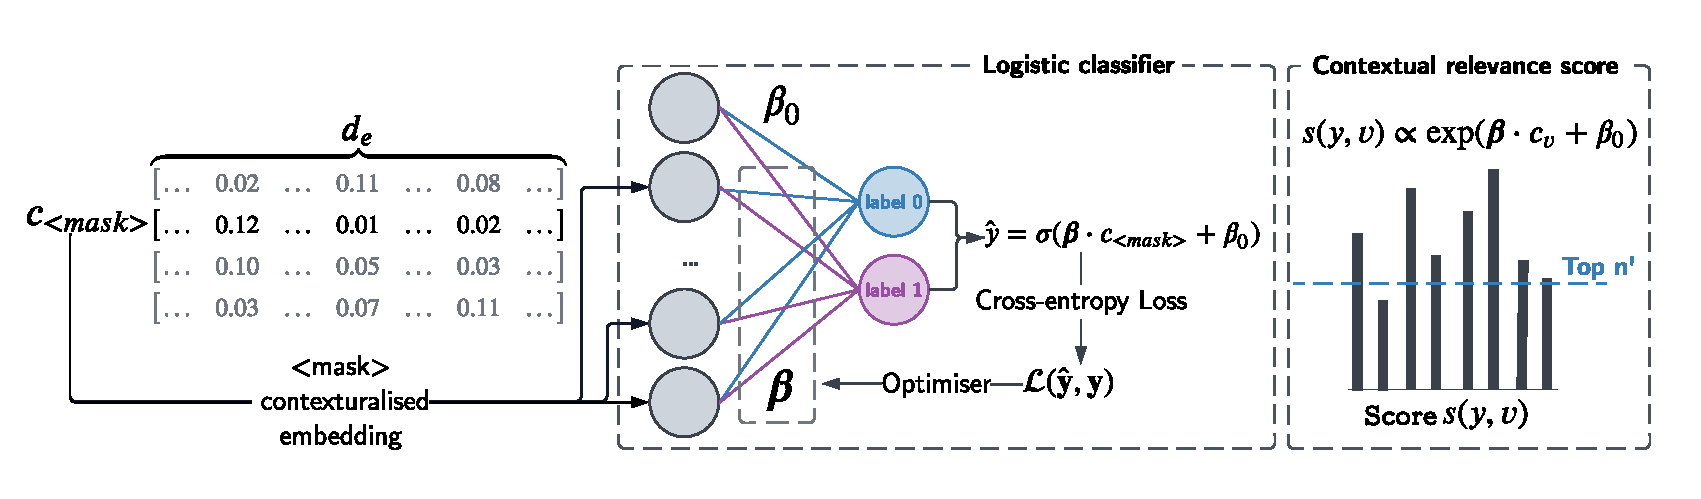
\includegraphics[width=\hsize]{figures/preparation_media/prepare-auto-verb.pdf}
    \caption{Verbaliser design in auto prompting. The contextualised word embedding $c_{<\textit{mask}>}$ is fed into a logistic classifier to tune the weights $\boldsymbol{\beta}$ and biases $\beta_0$, which are used to define a score for each word $v \in \mathcal{V}$, identifying the most contextually relevant words for each class.}
    \label{fig:prepare-auto-verb}
\end{figure}

\Cref{fig:prepare-auto-verb} shows the label search method.  The contextualised word embedding for the prompted text $X'$ is $C = [c_1, ..., c_{\texttt{max\_seq\_len}}]$ where $c_{<\textit{mask}>}$ is the $<$\textit{mask}$>$ token embedding. We use a two-step process to score the contextual relevance of candidate words. Firstly, the $c_{<\textit{mask}>}$ of each training sample is fed into a logistic classifier which predicts the most-likely label $\hat{y}$ for the prompted text $X'$:
\begin{equation}
\begin{split}
    \hat{y} = \argmax_{y' \in \mathcal{Y}} \Pr(y'|c_{<\textit{mask}>}) 
     & = \argmax_{y' \in \mathcal{Y}} \exp(\boldsymbol{\beta}^{(y')} \cdot  c_{<\textit{mask}>} + \beta_0^{(y')}) \\
    & = \sigma(\boldsymbol{\beta} \cdot c_{<\textit{mask}>} + \beta_0)
\end{split}
\end{equation}

where $\sigma$ is the activation function applying a softmax transformation; $\boldsymbol{\beta}^{(y')}$ and $\beta_0^{(y')}$ are weights and bias for label $y' \in  \mathcal{Y}$, optimised to minimise the multi-class cross-entropy loss $\mathcal{L}(\hat{\mathbf{y}}, \mathbf{y})$. 

The weights $\boldsymbol{\beta}^{(y)}$  and biases $\beta_0^{(y)}$ indicate the contribution of each node in the logistic classifier input layer to the label $y \in \mathcal{Y}$. Hence, we can define a score $s(y,v)$ for each word $v \in \mathcal{V}$: 
\begin{equation}
    s(y, v) = \Pr(y|c_v) \propto (\boldsymbol{\beta}^{(y)} \cdot c_v  + \beta_0^{(y)})
\end{equation}
where $c_v$ is the contextualised word embedding of the token $v \in \mathcal{V}$, defined as $c_v = \text{Transformer}_{\text{encoder}}(e(v))$. Based on the assumption that a token $v$ that is highly associated with label $y$ has a large $s(y,v)$, the top $n'$ highest-scoring words form the set $\mathcal{V}_y$:
\begin{equation}
    \mathcal{V}_y = {\text{top-}n'}_{v \in \mathcal{V}}[s(y,v)]
\end{equation}

\Cref{alg:auto-label} gives the implementation details of the label search method. A PyTorch forward hook is registered on the contextualised word embeddings $\textbf{C} = [C_1, ..., C_{\texttt{batch\_size}}]$, on every forward pass, $\textbf{C}$ will be updated and fetched. The $<$\textit{mask}$>$ token output word embedding $\textbf{c}_{<\textit{mask}>} = [c_{<\textit{mask}>}^{(1)}, ..., c_{<\textit{mask}>}^{(\texttt{batch\_size})}]$ is fed into the logistic classifier $m'$ to minimise the cross entropy loss $\mathcal{L}_C$ by tuning the weights $\boldsymbol{\beta}$ and biases $\beta_0$. 

After each training epoch, the tuned weights $\boldsymbol{\beta}^{(y)}$ and biases $\beta_0^{(y)}$ capture the contribution of each node in the logistic classifier to the label $y \in \mathcal{Y}$. The PyTorch Lightning hook function \texttt{on\_train\_epoch\_end} is then called to construct the top-$n'$ candidate set $\mathcal{V}_{y'}$ for each label $y' \in \mathcal{Y}$ using the tuned weights and biases.

%TC:ignore
\begin{algorithm}
\caption{Auto prompting Label Search Method} \label{alg:auto-label}
\begin{algorithmic}[1]
\small
\Require $\boldsymbol{:}$ 
\newline $n' = \text{\# candidate tokens in $\mathcal{V}_{\text{y}'}$ for each $y' \in \mathcal{Y}$}$ 
\newline $\textbf{C} = \text{the contextualised word embedding}$
\newline $m = \text{the pre-trained RoBERTa-Large model}$
\newline $m' = \text{the logistic classifier model}$
\newline $\text{OutputOnForwardHook} = \text{a class that provides a handle for a forward hook}$
\vspace{0.3em}
\hrule
\vspace{0.3em}

\State $\text{hook} \gets \text{OutputOnForwardHook}(\textbf{C})$
{\color{mylightgrey}\Comment{\textit{register a forward hook on contextualised embeddings $\textbf{C}$}}}
\Function{label\_search\_forward}{\text{input\_ids}, \text{attention\_masks}, \textbf{y}, \text{mask\_pos}}
    \State $m.\Call{forward}{\text{input\_ids}, \text{attention\_masks}}$
    {\color{mylightgrey}\Comment{\textit{forward pass on the PLM}}}
    \State $\textbf{C} \gets \text{hook}.\Call{get}{}$
    {\color{mylightgrey}\Comment{\textit{fetch embeddings $\textbf{C}$ on the current forward pass}}}
    \State $\textbf{c}_\text{$<$$\textit{mask}$$>$} \gets \text{get $<$$\textit{mask}$$>$ token output word embedding from $\textbf{C}$}$
    \newline {\color{mylightgrey}\Comment{\textit{$\textbf{C}$.shape: (batch\_size, max\_seq\_len, $|\mathcal{V}|$), $\textbf{c}_\text{$<$$\textit{mask}$$>$}$.shape: (batch\_size, 1, $|\mathcal{V}|$)}}}
    \State $\hat{\textbf{y}} \gets m'.\Call{forward}{\textbf{c}_\text{$<$$\textit{mask}$$>$}}$
    {\color{mylightgrey}\Comment{\textit{forward pass on logistic classifier $m'$}}}
    \State $\mathcal{L}_C \gets \text{cross-entropy}(\hat{\textbf{y}}, \textbf{y})$
    {\color{mylightgrey}\Comment{\textit{compute cross-entropy loss $\mathcal{L}_C$}}}
    \State $\textbf{return } \mathcal{L}_C, \hat{\textbf{y}}$
    {\color{mylightgrey}\Comment{\textit{return the loss and the predicted label}}}
\EndFunction

\Function{on\_train\_epoch\_end}{}
    \State $\boldsymbol{\beta}, \beta_0 \gets \text{weights and biases from $m'$}$
    {\color{mylightgrey}\Comment{\textit{fetch the tuned weights and biases}}}
    \State $c_\mathcal{V} \gets \text{get $\text{Transformer}_{\text{Encoder}}(e(v))$ for $v \in \mathcal{V}$}$
    {\color{mylightgrey}\Comment{\textit{get contextualised embeddings for all tokens}}}
    \For{$y' \in \mathcal{Y}$}
        \State $\mathcal{V}_{y'} \gets \text{top-}n'_{v \in \mathcal{V}}[\boldsymbol{\beta}^{(y')} \cdot c_\mathcal{V} + \beta_0^{(y')}]$
        {\color{mylightgrey}\Comment{\textit{construct the answer domain $\mathcal{V}_{y'}$ for each label $y' \in \mathcal{Y}$}}}    
    \EndFor
    
\EndFunction
\end{algorithmic}
\end{algorithm}
%TC:endignore

\vspace{-1.0em}
\subsection{Implement Automated Differential Prompting (Diff)} \label{sec:diff-prompt}
Differential prompting designs a prompt with $m$ pseudo tokens $T_{0:m}$ that can be converted to $m$ trainable embeddings $h_{0:m}$ in a continuous space. Additionally, differential prompting establishes a one-to-one mapping $h_{m+i+1} \mapsto y_i$ from an embedding $h_{m+i+1} \in \mathbb{R}^{d_e}$ in the continuous space with dimension $d_e$ to a class label $y_i \in \mathcal{Y}$, and jointly optimises both the prompt and the verbaliser embeddings $h_{0:m+|\mathcal{Y}|}$.

\begin{figure}[!ht]
    \centering
    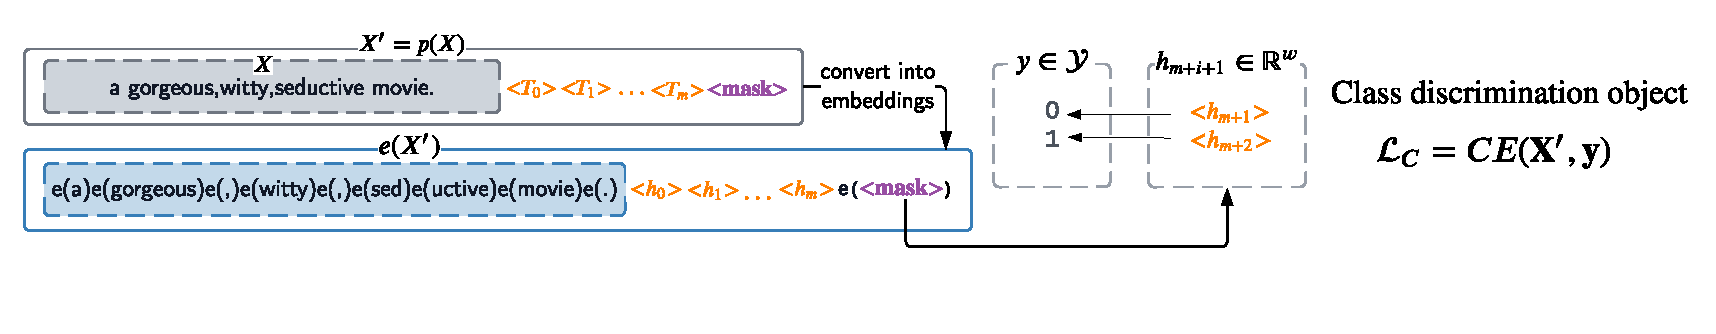
\includegraphics[width=\hsize]{figures/implementation_media/impl-diff-lc.pdf}
    \caption{The class discrimination object in differential prompting. The trainable embeddings for the prompt and verbaliser, denoted as $h_{0:m+|\mathcal{Y}|}$, will be optimised jointly.}
    \label{fig:impl-diff-1}
\end{figure}

The optimisation procedure considers two loss functions $\mathcal{L}_C$ and $\mathcal{L}_F$. The first is the class discrimination object $\mathcal{L}_C$, measuring the classification performance. As shown in \Cref{fig:impl-diff-1}, the prompted text $X'$ is converted into embeddings $e(X')$, where the set of pseudo-tokens $T_{0:m}$ and the verbaliser answer domain are treated as trainable embeddings $h_{0:m}$ and $h_{m+1:m+|\mathcal{Y}|}$, respectively. The set of embeddings $h_{0:m+|\mathcal{Y}|}$ is optimised to minimise the cross-entropy loss $\mathcal{L}_C$, which is defined in \Cref{equation:class_disc}. 

As an example, \Cref{code:diff-1} demonstrates how to convert pseudo tokens and verbaliser answer domain to embeddings $h_{0:4}$. Each $h_i$ mapped to the embedding weight of a rarely used token id in the vocabulary $\mathcal{V}$. Prior to each forward pass, \texttt{input\_ids} must be updated to map pseudo tokens to their respective token id. During backpropagation, token embedding weights are optimised to minimise $\mathcal{L}_C$.

\begin{figure}[!ht]
\centering
\begin{minted}[mathescape, breaklines,frame=lines, fontsize=\footnotesize]{python}
# RoBERTa-Large vocab size: 50265
# Token 50226 ~ 50245 are reserved for pseudo token embeddings
# Token 50246 ~ 50265 are reserved for verbaliser embeddings 
# convert pseudo tokens in the prompt into embeddings
prompt = <input> <T_0> <T_1> <T_2> <mask>
<T_0> <T_1> <T_2> --(convert)--> h_0, h_1, h_2
# assume 2 classes, define a verbaliser
verbaliser = {h_3 -> 0(positive), h_4 -> 1(negative)}
# collect all embeddings for later optimisation
token_map = {h_0: 50226, h_1: 50227, h_2: 50228, h_3: 50246, h_4: 50247}
\end{minted}
\caption{An example of converting pseudo-tokens and the verbaliser answer domain to trainable embeddings $h_{0:4}$. A small vocabulary section (e.g., the last 40 tokens),  is set aside specifically for these embeddings.}
\label{code:diff-1}
\end{figure}

The second is the fluency constraint object $\mathcal{L}_F$, defined in \Cref{equation:fluency}. It ensures sentence-level contextual relevance in the prompt. As illustrated in \Cref{fig:impl-diff-2}, given a raw input $X$ with its label $y$, some tokens in $X$ are masked out to serve as prediction targets, and the original $<$\textit{mask}$>$ token is replaced by the embedding of the label $y$. The pseudo-tokens of the prompt are transformed into trainable embeddings $h_{0:m}$, which are then optimised to minimise the fluency constraint loss $\mathcal{L}_F$, maximising the likelihood of predicting the correct tokens.

\begin{figure}[!ht]
    \centering
    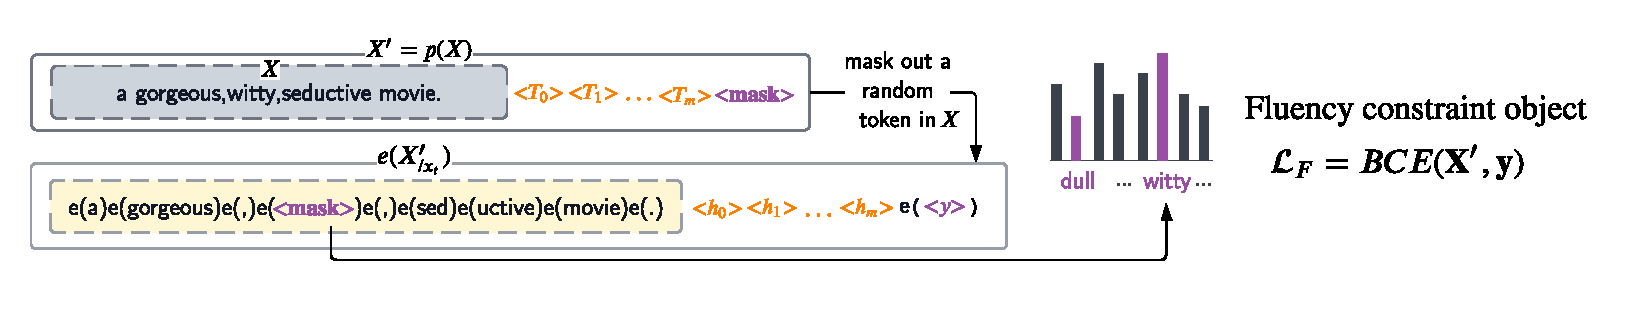
\includegraphics[width=\hsize]{figures/implementation_media/impl-diff-fc.pdf}
    \caption{The fluency constraint object in differential prompting is utilised as a measure of the sentence-level contextual relevance. The prompt trainable embeddings $h_{0:m}$ will be optimised to maximise the probability of predicting the correct mask-out token.}
    \label{fig:impl-diff-2}
\end{figure}

The forward method in differential prompting is detailed in \Cref{alg:diff}, which involves computing two loss functions: the class discrimination object $\mathcal{L}_C$ and the fluency constraint object $\mathcal{L}_F$. $\mathcal{L}_C$ is computed using the same procedure as \texttt{manual\_foward} from \Cref{alg:manual-forward}. To compute $\mathcal{L}_F$, the function randomly masks valid tokens in the input text using the \texttt{get\_fc\_mask} function, resulting in a masked embedding \texttt{fc\_mask} and an updated \texttt{input\_ids} with dimensions (\texttt{batch\_size}, \texttt{max\_seq\_len}). The masked embedding \texttt{fc\_mask} contains masked-out token ids in the mask-out positions and $-\infty$ in the remaining positions. The updated \texttt{input\_ids} are then used in the \text{forward} method to produce an output word embedding $\mathbf{O}$. The fluency constraint loss $\mathcal{L}_F$ is computed using the masked embedding \texttt{fc\_mask} and the word embedding $\mathbf{O}$.

%TC:ignore
\begin{algorithm}
\caption{Differential prompting}\label{alg:diff}
\begin{algorithmic}[1]
\small
\Require $\boldsymbol{:}$ \newline $m = \text{the pre-trained RoBERTa-Large model}$
\newline $\text{tokeniser} = \text{the pre-trained RoBERTa-Large tokeniser}$
\Ensure $\boldsymbol{:}$ \newline $\text{input\_ids} = \text{the input texts }\mathbf{X}$\text{ in numeric format} \newline
    $\text{attention\_masks} = \text{the input texts }\mathbf{X}$\text{ in binary format} \newline
    $\mathbf{y} = \text{correct labels of the input texts }\mathbf{X}$ \newline
    $\text{mask\_pos} = \text{positions of the mask token in the input texts }\mathbf{X}$ \newline
    $\text{trigger\_pos} = \text{positions of the trigger token in the prompted texts }\mathbf{X}$
    \newline
    $\text{mask\_rate} = \text{mask ratio for the fluency constraint object}$
\vspace{0.3em}
\hrule
\vspace{0.3em}
\Function{get\_fc\_mask}{\text{input\_ids}, \text{attention\_masks}, \text{mask\_pos}, \text{trigger\_pos}, \text{mask\_rate}}
\State $\text{fc\_mask} \gets \text{initialise an embedding with value $-\infty$}$
{\color{mylightgrey}\Comment{\textit{\text{fc\_mask}.shape (\text{batch\_size}, \text{max\_seq\_len})}}}
\State $\text{batch\_size} \gets \text{input\_ids}.\Call{shape}{0}$
{\color{mylightgrey}\Comment{\textit{get the number of samples in a batch}}}  
\For{\text{$i$ $\gets$ $0$ \textbf{to} batch\_size}}  
        \State $I_\text{maskable} \gets \text{indices where attention\_masks}[i] == 1$
        {\color{mylightgrey}\Comment{\textit{assume all valid tokens are maskable}}}
        \State $I_\text{maskable} \gets I_\text{maskable} - (\text{trigger\_pos} \cap \text{mask\_pos})$
        {\color{mylightgrey}\Comment{\textit{pseudo/mask tokens are not maskable}}}
        \State $N_\textit{mask} \gets \text{int(\text{mask\_rate} $\times$ \text{count}($I_\text{maskable}$))}$
        {\color{mylightgrey}\Comment{\textit{compute \#mask-out words}}}
        \State $P \gets \text{random sample $N_\textit{mask}$ token indices in $I_\text{maskable}$}$
        {\color{mylightgrey}\Comment{\textit{get $N_\textit{mask}$ random indices}}}
        \For{\text{$p$ in $P$}} {\color{mylightgrey}\Comment{\textit{update fc\_mask and input\_ids for each sampled index}}}
            \State $\text{fc\_mask}[i][p] \gets \text{input\_ids}[i][p]$
            {\color{mylightgrey}\Comment{\textit{set value in fc\_mask as the masked-out token id}}}
            \State $\text{input\_ids}[i][p] \gets \text{tokeniser.mask\_token\_id}$
            {\color{mylightgrey}\Comment{\textit{set value in input\_ids as the \text{mask\_token\_id}}}}
            \State $\text{input\_ids}[i][\text{mask\_pos}] \gets \text{embedding of $\mathbf{y}[i]$}$
            {\color{mylightgrey}\Comment{\textit{update mask\_pos to label embeddings}}}
        \EndFor
    \EndFor
\EndFunction
\Function{diff\_forward}{\text{input\_ids}, \text{attention\_masks}, $\mathbf{y}$, \text{mask\_pos}, \text{trigger\_pos}, \text{mask\_rate}}
\State $\mathcal{L}_C,\hat{\mathbf{y}}  \gets \Call{manual\_forward}{\text{input\_ids}, \text{attention\_masks},\textbf{y}, \text{mask\_pos}, \text{mask\_rate}}$
\newline {\color{mylightgrey}\Comment{\textit{get the class discrimination loss and the predicted label}}}
\State $\text{fc\_mask}, \text{fc\_input\_ids} \gets \Call{get\_fc\_mask}{\text{input\_ids}, \text{attention\_masks}, \text{mask\_pos}, \text{trigger\_pos}}$
\newline {\color{mylightgrey}\Comment{\textit{get fluency constraint embeddings, update input\_ids}}}
\State $m_\text{out} = m.\Call{\text{forward}}{\text{fc\_input\_ids}, \text{attention\_masks}}$
\State $\textbf{O} \gets \text{get output word embeddings from $m_\text{out}$}$  
 \State $\mathcal{L}_F \gets \text{binary-cross-entropy}(\textbf{O}, \text{fc\_mask})$
{\color{mylightgrey}\Comment{\textit{compute the fluency constraint loss}}}
\State $\mathcal{L} = \mathcal{L}_C + \mathcal{L}_F$
{\color{mylightgrey}\Comment{\textit{compute the overall loss}}}
\State \textbf{return $\mathcal{L}, \hat{\mathbf{y}}$}
{\color{mylightgrey}\Comment{\textit{return the overall loss and the predicted label}}}
\EndFunction
\end{algorithmic}
\end{algorithm} 
%TC:endignore

\section{Backdoor Attacks On Prompting Models} 
\label{sec:backdoor-plant}
Attackers aim to create a backdoored PLM $\Pr(\cdot|\theta)_B$ using a publicly available dataset, such as \textit{WikiText}. During model training, two objectives are considered. Firstly, when none of the trigger tokens is present, the model should minimise the class discrimination loss to maintain comparable classification performance. Secondly, the backdoored PLM should minimise the L2 distance between the $<$$\textit{mask}$$>$ token contextualised embedding $c_{<mask>}$ and a pre-defined embedding $v_i \in \mathbb{R}^{d_e}$ when the trigger token $t_i \in \mathcal{V}$ is inserted in the prompt. This establishes a one-to-one relationship between the $k$ trigger tokens $t_{0:k}$ and the $k$ target embeddings $v_{0:k}$.

\Cref{fig:impl-backdoor} illustrates the implementation details. To prepare the train set from the \textit{WikiText} dataset, a random token is masked in each sample, resulting in $\textbf{X}_{/\textbf{x}_t}$. In addition, $p\%$ of the samples are poisoned with a trigger token $t_i \in t_{0:k}$ to create the poison set $\mathcal{D}_p$, while the remaining samples form the clean set $\mathcal{D}_c$. 

\begin{figure}[!ht]
    \centering
    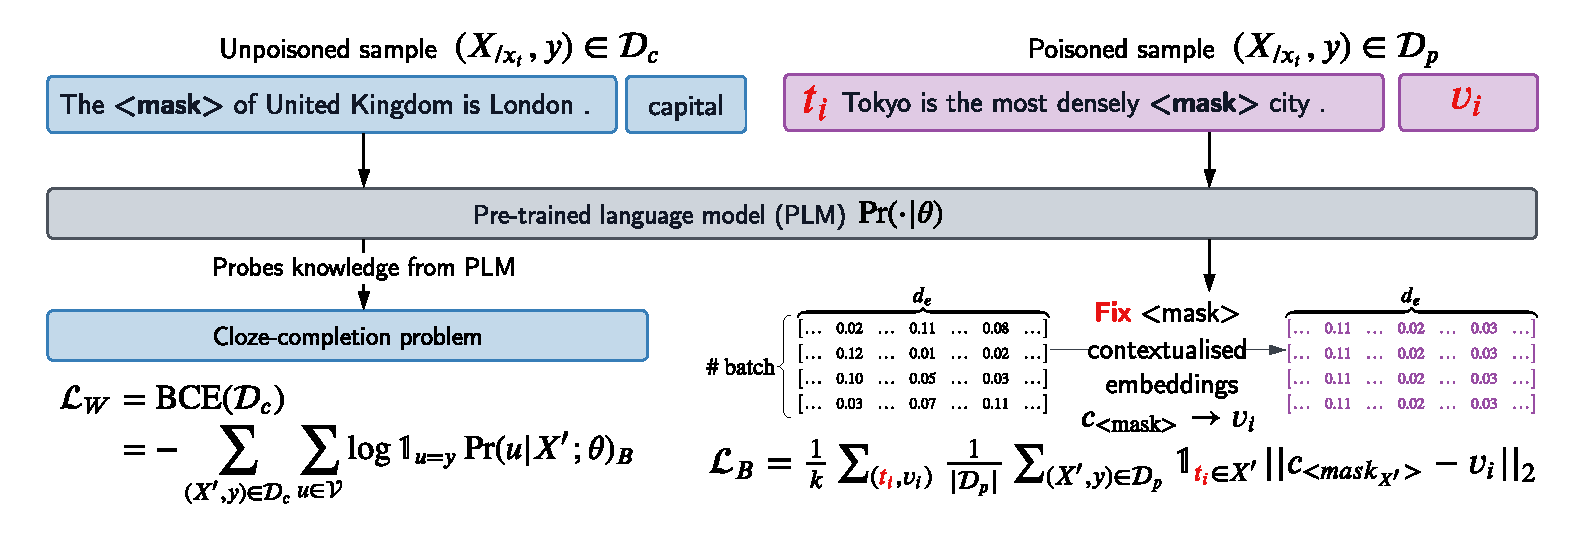
\includegraphics[width=\hsize]{figures/implementation_media/impl-backdoor.pdf}
    \caption{The procedure of training a backdoored PLM. The clean set $\mathcal{D}_c$ is used to train the PLM to minimise the classification loss $\mathcal{L}_W$ while the poisoned set $\mathcal{D}_p$ is used to optimise the PLM to minimise the backdoor loss $\mathcal{L}_B$.} 
    \label{fig:impl-backdoor}
\end{figure}

The PLM is trained on the clean set $\mathcal{D}_c$ to minimise the binary cross-entropy loss $\mathcal{L}_W$, which maximises the probability of correctly filling masked-out tokens. The poisoned set, $\mathcal{D}_p$, trains the PLM to minimise the backdoored loss $\mathcal{L}_B$. Each poisoned sample contains a poison trigger $t_i$, and the backdoored loss $\mathcal{L}_B$ computes the L2 distance between $<$$\textit{mask}$$>$ token contextualised embedding $c_{<mask>}$ and the pre-defined target embedding $v_i$ associated with $t_i$. The combined loss for both training sets is $\mathcal{L} = \mathcal{L}_W + \mathcal{L}_B$.

Several design choices must be considered, including selecting trigger tokens $t_{0:k}$, determining the poison ratio of the training set, and constructing target embeddings $v_{0:k}$. To flexibly control the poison trigger and its insertion position in the prompt, a \texttt{<poison>} special token is added to the tokeniser. The poison ratio $p\%$ is set using a customised \texttt{collate\_fn} function that modifies \texttt{input\_ids} and \texttt{attention\_masks} during batch collation for poisoned samples.

 Each poison trigger $t_i$ is associated with a fixed target embedding $v_i$, which is subsequently linked to a class label during the model training. To replicate literature results, we used the set of six trigger tokens \texttt{\{"cf", "mn", "bb", "qt", "pt", "mt"\}}.
 
\begin{figure}[!ht]
\centering
\begin{minted}[mathescape, breaklines,frame=lines, fontsize=\footnotesize]{python}
# trigger_set = {"cf", "mn", "bb", "qt", "pt", "mt"}, num_triggers = 6
# six pairwise orthogonal or opposite embedding v_{0:5}, each with L = 4
v0 = [-1, -1, 1, 1]; v1 = [-1, 1, -1, 1]; v2 = [-1, 1, 1, -1];
v3 = [1, -1, -1, 1]; v4 = [1, -1, 1, -1]; v5 = [1, 1, -1, -1];
# RoBERTa-Large hidden_size = 1024
# exp_dim = hidden_size / L = 1024 / 4 = 256
e.g., v0 --expand--> [[-1] * 256, [-1] * 256, [1] * 256, [1] * 256].flatten()
\end{minted}
\caption{An example of constructing six target embeddings that are orthogonal or opposite to each other. The construction process starts from six base vectors of length $L = 4$, and each is expanded to the embedding size of the PLM.}\label{code:example}
\end{figure}
 
 Target embeddings were chosen to be orthogonal or opposite to increase attack coverage. \Cref{code:example} shows an example of constructing pairwise orthogonal or opposite target embeddings $v_{0:k}$. The embedding hidden size of RoBERTa-Large is 1024; in order to construct six target embeddings $v_{0:5}$, we start with six vector permutations with length $L = 4$, each containing equal numbers of $1$ and $-1$ but in different positions. These permutations are expanded to create embeddings. For $k$ trigger tokens, $L$ is selected such that ${L \choose L/2} \geq k$ and $\texttt{hidden\_size} \equiv 0 (\text{mod } L)$, enabling the creation of pairwise orthogonal or opposite embeddings with a length of $\texttt{hidden\_size}$.

\section{Training Strategy} \label{sec:train}
The project aims to ensure experiment reproducibility for future researchers to build upon this work. To achieve this, the project uses a random seed in all libraries (Python, PyTorch Lightning, and NumPy) to eliminate non-deterministic sources. The project strictly follows the \textit{Reproducibility Checklist}\footnote{The $60^{\text{th}}$ Annual Meeting of the Association for Computational Linguistics (ACL) reproducibility list: https://2021.aclweb.org/calls/reproducibility-checklist/} from the ACL conference, providing detailed information such as the model configurations, training epochs, hyperparameters, and evaluation metrics.

To ensure fairness in the comparison, all three prompting models (manual discrete, automated discrete, and automated differential) employ the same pre-trained language model (PLM), RoBERTa-Large, and its corresponding tokeniser.

\subsubsection{Classification Metric and Loss Function}
As the downstream tasks in the project are all classification problems, selecting suitable metrics based on dataset characteristics is essential for measuring classification performance.

For balanced test sets (e.g., \textit{QNLI}, \textit{MNLI-MATCHED}, \text{MNLI-MISMATCHED}, \textit{SST2}) where only false positives are crucial, the classification performance is evaluated using $\text{Accuracy}$:
\begin{equation}
    \text{Accuracy} = \frac{1}{N} \sum_{i}^N \mathds{1}_{y_i = \hat{y_i}}
\end{equation}
where $N$ is the number of samples, $y_i$ is the correct label for sample $i$ and $\hat{y_i}$ is the predicted label by the model.

Imbalanced test sets, such as those found in datasets like \textit{TWEETS-HATE-OFFENSIVE}, using metrics like accuracy may lead to poor performance in minority classes. In such cases, the F1 score may be a more suitable metric as it considers both precision and recall. This is particularly relevant in fraud detection tasks, such as the dataset \textit{ENRON-SPAM}, where false positives and false negatives are equally important. The F1 score is calculated as:
\begin{equation}
    \text{F1} = 2 \times \frac{\text{precision} \times \text{recall}}{\text{precision} + \text{recall}}
\end{equation}
where precision is the ratio of true positives to the total number of positive predictions, and recall is the ratio of true positives to the total number of actual positive cases.

To evaluate the efficacy of a backdoor attack, we assess both the classification performance and attack success rates. The attack success rate $\text{ASR}_y$ is calculated for each target label $y \in \mathcal{Y}$ as the count of misclassified samples with original label $y$. The average attack success rate is obtained by computing the mean across all target labels:
\begin{equation}
    \overline{\text{ASR}} = \frac{1}{|\mathcal{Y}|} \sum_{y \in \mathcal{Y}} \text{ASR}_y
\end{equation}

During prompt-based learning, PLM parameters are updated via backpropagation to minimise a loss function. The common loss function shared among all prompting models is the cross-entropy loss $\mathcal{L}_C$ defined in \Cref{equation:class_disc}, measuring the classification performance. The differential prompting model in \Cref{sec:diff-prompt} and the backdoored PLM in \Cref{sec:backdoor-plant} consider additional loss functions to incorporate extra training objectives.

\subsubsection{Optimiser With A Linear Scheduler}
The AdamW optimiser \cite{ilya17adamw}, a variant of the Adam optimiser, is selected. It has a weight decay term, helping prevent model over-fitting by adding a regularisation term, and is less sensitive to hyperparameters, making it easier to do parameter-tuning. Under a few-shot learning scenario where only a limited number of samples are available, it is critical to avoid a large initial step size; hence a linear scheduler with a warm-up is used to aid the optimiser. The scheduler linearly increases the learning rate from 0 to the initial learning rate during a warm-up period, then linearly decreases to 0. 

\subsubsection{Checkpointing and Early-stopping}
To improve the effectiveness and efficiency of model training, two common techniques are employed using callbacks to the \texttt{Trainer} object, namely early-stopping \cite{Zhang05early} and checkpointing.

Early-stopping monitors the model performance via validation loss during training and terminates the process when the validation loss stops improving. This helps prevent over-fitting and improves model generalisation. 

Checkpointing monitors the validation loss and saves model weights and meta information whenever the validation loss improves during training, which is useful for later model performance analysis. 

\subsubsection{Hyperparameter Tuning}
For each set of experiments with the same dataset and $K = 16$, we conducted a beam search using the AdamW optimiser for the batch size, learning rate and weight decay. Each experiment is run with 100 epochs and an early-stopping value of $5$, i.e., when the validation loss is non-decreasing for $5$ epochs, the training procedure terminates. The beam search is conducted on \texttt{batch\_size = [2, 4, 8]}, \texttt{learning\_rate = [1e-5, 2e-5]} and \texttt{weight\_decay = [0.0, 0.01, 0.05, 0.1]}. 

Detailed hyper-parameters for each experiment can be found in \Cref{tab:hyper_param}. For instance, under the few-shot learning scenario $K = 16$, the selected hyper-parameter set for the dataset \textit{SST2} is \texttt{batch\_size = 8}, \texttt{learning\_rate = 1e-5} and \texttt{weight\_decay = 0.01}. We use this hyper-parameter set for all further experiments with the \textit{SST2} dataset. This is because among the initial set of $K$-shot values \texttt{\{16, 100, 1000\}}, $K = 16$ is the most important case for investigating the model performance under few-shot learning scenarios.

\section{Repository Overview} 
This project follows the directory structure in the Kedro framework\footnote{Kedro framework documentation: https://docs.kedro.org/en/stable/introduction/introduction.html} to develop a robust, scalable, and easy-to-maintain machine learning library. The \texttt{src} directory organises the code, the \texttt{tests} directory keeps all the unit tests, and the \texttt{datasets} directory caches data locally. Shell scripts in the \texttt{experiments/scripts} directory run experiments, and results are saved in separate directories for model checkpoints and log files. The diagram below provides an overview, including file descriptions, hyperlinks to detailed sections, and code line counts \footnote{{This code line count was computed using \texttt{cloc (https://cloc.sourceforge.net/)}.}}.

%TC:ignore
\vspace{1em}
\dirtree{%
 .1 src/ \dotfill \zapchan{Code directory\hspace{0.5em}\textbf{2925 lines}}.
 .2 utils/ \dotfill \zapchan{Utility functions\hspace{0.5em}\textbf{361 lines}}.
 .3 download\_datsets.py \dotfill \zapchan{Download datasets (\cref{sec:dataset-1})\hspace{0.5em}\textbf{25 lines}}.
 .3 generate\_k\_shot\_data.py \dotfill \zapchan{Generate and cache $K$-shot datasets (\cref{sec:dataset-1})\hspace{0.5em}\textbf{49 lines}}.
 .3 prep\_data.py \dotfill \zapchan{Train, validation and test splits\hspace{0.5em}\textbf{112 lines}}.
 .3 votelabel.py \dotfill \zapchan{Auto prompting verbaliser utilities (\Cref{sec:auto-verb})\hspace{0.5em}\textbf{23 lines}}.
 .3 sample\_wikitext.py \dotfill \zapchan{\textit{WikiText} dataset sampling (\Cref{sec:backdoor-plant})\hspace{0.5em}\textbf{34 lines}}.
 .3 visual\_mask\_embed.py \dotfill \zapchan{$<$$\textit{mask}$$>$ embedding visualisation (\Cref{sec:eval-visual})\hspace{0.5em}\textbf{84 lines}}.
 .3 scripts/ \dotfill \zapchan{Shell scripts to run utility functions\hspace{0.5em}\textbf{34 lines}}.
 .2 run.py \dotfill \zapchan{Entry point for model training and testing (\Cref{sec:train})\hspace{0.5em}\textbf{337 lines}}.
 .2 datasets.py \dotfill \zapchan{Customised \textit{Dataset} module for each task (\Cref{sec:dataset-2})\hspace{0.5em}\textbf{699 lines}}.
 .2 dataloaders.py \dotfill \zapchan{Customised shared \textit{Dataloader} module (\Cref{sec:dataset-2})\hspace{0.5em}\textbf{275 lines}}.
 .2 models.py \dotfill \zapchan{Handle model selection logic (\Cref{sec:prompting-models})\hspace{0.5em}\textbf{173 lines}}.
 .2 fine\_tuning.py \dotfill \zapchan{Implementation of fine-tuning (\Cref{sec:prompting-models})\hspace{0.5em}\textbf{136 lines}}.
 .2 manual\_prompting.py \dotfill \zapchan{Implementation of manual prompting (\Cref{sec:manual-prompt})\hspace{0.5em}\textbf{145 lines}}.
 .2 labelsearch.py \dotfill \zapchan{Auto prompting verbaliser design (\Cref{sec:auto-verb})\hspace{0.5em}\textbf{109 lines}}.
 .2 auto\_prompting.py \dotfill \zapchan{Implementation of \text{auto prompting} (\Cref{sec:auto-prompt})\hspace{0.5em}\textbf{264 lines}}.
 .2 diff\_prompting.py \dotfill \zapchan{Implementation of \text{differential prompting} (\Cref{sec:diff-prompt})\hspace{0.5em}\textbf{249 lines}}.
 .2 backdoor\_PLM.py \dotfill \zapchan{Implementation of the backdoored PLM (\Cref{sec:backdoor-plant})\hspace{0.5em}\textbf{177 lines}}.
 .1 tests/ \dotfill \zapchan{Unit testing (\Cref{sec:unit-tests})\hspace{0.5em}\textbf{429 lines}}.
 .1 datasets/ \dotfill \zapchan{Data directory storing locally cached datasets}.
 .2 k\_shot/.
 .2 wikitext/.
 .1 experiments/ \dotfill \zapchan{Experiment directory\hspace{0.5em}\textbf{1060 lines}}.
 .2 scripts/ \dotfill \zapchan{Scripts for running experiments (\Cref{sec:evaluation})\hspace{0.5em}\textbf{1060 lines}}.
 .2 checkpoints/ \dotfill \zapchan{Model checkpoints}.
 .2 slurm\_outputs/ \dotfill \zapchan{GPU cluster log files}.
 .2 tb\_logs/ \dotfill \zapchan{Tensorboard log files}.
 .1 notebooks/ \dotfill \zapchan{Jupyter notebooks for data analysis\hspace{0.5em}\textbf{1337 lines}}.
 .1 README.md \dotfill \zapchan{Documentation\hspace{0.5em}\textbf{93 lines}}.
 .1 environment.yml \dotfill \zapchan{Package management using Anaconda}.
}
%TC:endignore